\chapter{Method}
\label{ch:method}

\section{Datasets}
\label{ch:method-dataset} This project focused on building an automated
segmentation solution for radiotherapy. Two applications were targeted: A
multi-organ segmentation model for pelvic imaging (with patient, bladder and
rectum contouring); and a single structure model for vacuum bag contouring in
canine imaging. Anonymised pelvic imaging data was provided by Riverina Cancer
Care Centre from active prostate cancer RT patients over multiple stages of
treatment. Canine imaging data was provided by the Small Animal Specialists
Hospital (SASH) and contained variable cancer locations and patient
orientations. All input data consisted of raw diagnostic CT images acquired with
a 512 x 512 matrix. Pelvic imaging scans were comprised of 1.37 mm x 1.37 mm x 2
mm voxels; while canine imaging scans contained variable spacings across
patients, with an average voxel size of 0.85 mm x 0.85 mm x 1.91 mm.

Patient scans were exported from the Monaco treatment planning system to DICOM
format, from which image-structure pairs were extracted, transformed from
patient-space to a non-dimensional matrix-space, and saved individually as model
input-output arrays for further processing. Initial modelling was attempted with
contours extracted on-the-fly from DICOM files; however, this resulted in a
significant CPU bottleneck which limited GPU capacity during training.

In addition, any advantage of removing the intermediate file processing step
(DICOM to array) was made redundant upon determining that significant data
cleaning would be required for contour consistency. For instance, vacuum bag
segmentation was often incomplete in patient scans, as only clinically relevant
locations included full contouring; this may satisfy clinical requirements,
however, consistent labels are required for machine learning. The final data
pipeline was designed to handle filenames (pointing to arrays) as the primary
method of matching an input with the ground truth. Each filename was read into
memory if it belonged to the current batch; removing memory constraints on
dataset size, as only a single batch populated the RAM at each training step.

A total of 15 patients were used for pelvic imaging, corresponding to 1991 total
input instances. Data was split at the patient level to enforce independence
across training, validation and test datasets. 12 patient scans were used for
training, while validation and testing used 2 and 1, respectively. The complete
data distribution is provided in Table \ref{table:data_prostate}. Patient
contours were present in all input data, while the bladder was present in 28\%
of slices, and rectum in 37\%. A significant pixel-wise class imbalance existed
between structures in pelvic imaging, as the multi-organ segmentation output
space was 512 x 512 x 3. Patient pixels corresponded to a total of 5.2\% of all
output pixel in the data, with 0.08\% and 0.02\% corresponding to bladder and
rectum.

\begin{table}[H]
\footnotesize
\caption{Data distribution for pelvic imaging.}
\centering
\begin{tabular}{c c c c c}
\hline\hline
& Training & Validation & Testing & Total  \\ [0.5ex]
\hline

Images(Patients) & 1751(12) & 282(2) & 138(1) & 1991(15) \\
 \\
 \hline\hline
		 & Images total (\%) & Pixel-image ratio (\%)& Pixel-output ratio (\%) & Pixels total (\%)\\ [0.5ex]
\hline
Patient  & 100 & 15.6  &  5.21 & 5.21\\
Bladder  & 28.0 & 0.862 & 0.287 & 0.081\\
Rectum   & 37.0 & 0.172 & 0.057 & 0.021\\
\hline\hline
\end{tabular}
\label{table:data_prostate}
\end{table}


For vacuum bag segmentation, a total of 26 patients were used, with 21, 3, and 2
corresponding to training, validation and testing, respectively. Vacuum bag
structures were present in 70\% of total input images, as seen in Table
\ref{table:data_vet}.

\begin{table}[H]
\footnotesize
\caption{Data distribution for canine imaging.}
\centering
\begin{tabular}{c c c c c}
\hline\hline
& Training & Validation & Testing & Total  \\ [0.5ex]
\hline

Images(Patients) & 1912(21) & 340(3) & 187(2) & 2439(26) \\
 \\
 \hline\hline
		 & Images total (\%) & Pixel-image ratio (\%)& Pixel-output ratio (\%) & Pixels total (\%)\\ [0.5ex]
\hline
Vacbag   & 70.0& 13.4  & 13.4  &  9.4 \\

\hline\hline
\end{tabular}
\label{table:data_vet}
\end{table}



Significant data augmentation was used to increase the effective size of our
dataset and to aid dropout regularisation in the reduction of over-fitting.
Augmentation was performed on-demand for each input-output pair in a batch, and
sampled from a random uniform distribution with probability listed below for
each type. 50\% of total training data was selected for augmentation per epoch.
Augmentations included: Left-right image inversion ($P_{val}=0.5$), random image
cropping and resizing ($P_{val}=0.33$, minimum crop size 500 x 500), elastic
deformations ($P_{val}=0.33$, with ($\alpha$, $\sigma$) pairs selected from
(1201, 10), (1501, 12), and (991, 8)), affine transformations ($P_{val}=0.33$,
$\alpha_{max}=20$), and Gaussian noise ($P_{val}=0.33$, $\mu=0$,
$\sigma_{max}=0.3$). Furthermore, all input data (including test data) was
normalised with respect to the training and validation distributions prior to
augmentation. Randomly sampled transformations are included in Figure
\ref{fig:augment}.

\begin{figure}[h]
	\begin{center}
		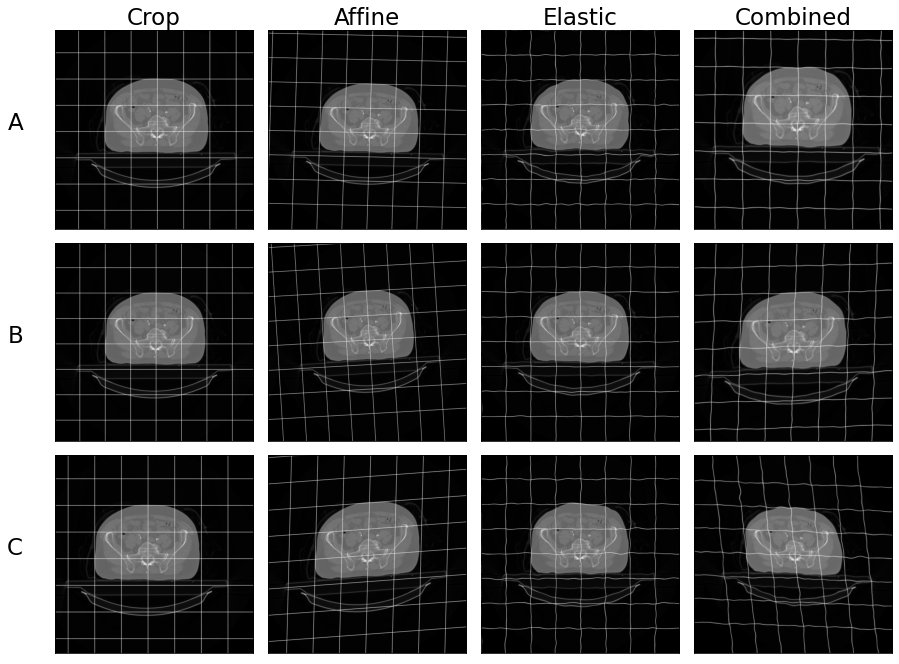
\includegraphics[width=1\textwidth]{figures/augment}
		\caption{Training data augmentation for a single input image with random
      sampling of parameters: image crop and resize, affine transformation,
      elastic deformation, and combined transformations. Each matching contour
      set is augmented under an identical transformation. An individual
      transformation type has $P_{val}=0.33$ of occurring. Additional
      augmentations not shown: Left/right inversion and Gaussian noise.}
		\label{fig:augment}
	\end{center}
\end{figure}

\section{Model architecture}
\label{ch:method-architecture} A 2D U-Net architecture was designed with 7
levels, consisting of 6 encoding and 6 decoding blocks, outlined in Figure
\ref{fig:model}. The model accepts a full resolution (512 x 512) CT image as
input, and outputs selected contours in the original resolution by the use of
padded convolutions, each of which is followed by batch normalisation and ReLU
activation. Each encoding block performs a repeated sequence of 3 x 3
convolution (increasing feature channels). Extracted feature maps are passed via
the skip connection in one pathway, while a 3 x 3 convolution with a stride size
of 2 results in the halving of resolution, before features are passed to the
next encoding block.

Conversely, each decoding block upsamples input via a 3 x 3 2D transposed
convolution with stride size of 2. Upsampled feature maps are then concatenated
with skip connections. Dropout is selectively performed with a probability value
of 20\%, before additional 3 x 3 convolution sequences reduce the feature
channels. Finally, multi-organ segmentation can be controlled via the C output
variable, corresponding to the number of segmentations (or channels) specified
in the final 1 x 1 convolutional layer. A sigmoid activation function is used to
account for the non-mutually exclusive nature of pixel-wise binary
classification on anatomic structures (i.e. a voxel can belong to multiple
structures).

\begin{figure}[h]
	\begin{center}
		\hspace*{-1.3cm}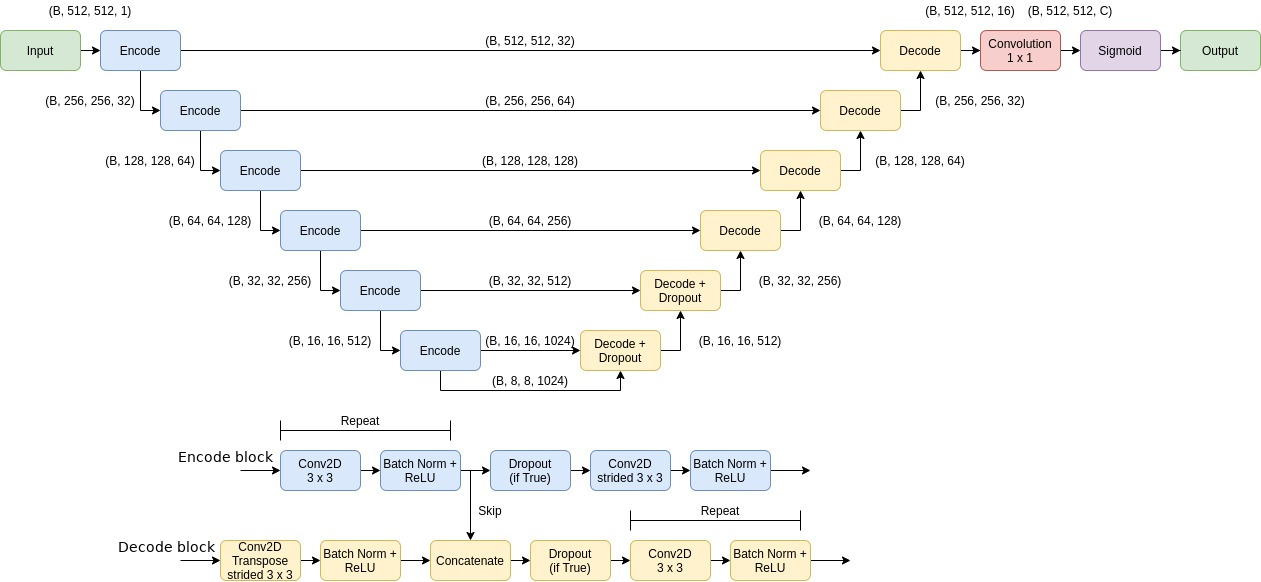
\includegraphics[width=1.15\textwidth]{figures/model_diagram}
		\caption{Modified 2D U-Net architecture: Composed of encoding (blue) and
      decoding blocks (yellow). MaxPooling layers are replaced by strided
      convolution. Addition of batch normalisation and final sigmoid activation.
      Tensor dimensions (Batch size, X, Y, Channels) are included for each
      connection. Internal layers of encoding blocks (blue) and decoding blocks
      (yellow) are included below the high-level overview.}
		\label{fig:model}
	\end{center}
\end{figure}

The model was trained using the Adam (Adaptive momentum estimation) optimisation
algorithm \cite{kingma2014} with an initial learning rate of $10^{-5}$, a batch
size of 1 for pelvic imaging, and 3 for canine imaging. Model training was
scheduled to conclude when validation loss had not improved for a period of 20
epochs. In addition, learning rate decay ($\alpha /2$) was triggered by a validation loss
plateau period of 3 epochs. Initial model weights were determined via `He'
kernel initialisation), which samples from a zero mean Gaussian distribution
with variance $\sigma=\sqrt{2/N}$ (as in Ronneberger et al
\cite{Ronneberger_2015}), where N is the incoming nodes for a single activation
(i.e. for n x n convolution over M feature maps, N = n x n x M). In addition,
training for pelvic imaging was accelerated by adopting the strategy of Bertels
et al., to further initialise model parameters via 3 epochs of training with
binary cross entropy \cite{Bertels2019}.

A total of 5 loss functions were assessed for pelvic imaging: Binary Cross
entropy (BCE), soft dice similarity coefficient (soft DSC) \cite{Bertels2019},
weighted soft dice similarity coefficient (w. soft DSC or generalised dice loss)
\cite{Sudre_2017}, a combination loss BCE + 2 (w. soft DSC)
\cite{taghanaki2018}, and focal Tversky loss \cite{Zhu_2018, Khan2019,
abraham2018}. In contrast, weighted soft DSC was not attempted for canine
imaging due to the single segmentation output. Weights for the w. soft DSC were
inversely proportional to the number of positive pixels in each ground truth
segmentation (as described by Sudre et al. \cite{Sudre_2017}) - forcing the
model to place a higher priority on infrequent or relatively smaller OARs
\cite{Sudre_2017}. Focal Tversky loss (as described in Khan et al.
\cite{Khan2019}) was calculated with $\gamma = \frac{4}{3}$, $\alpha=0.7$, and
$\beta=0.3$, as this was reported to produce the highest performance in the
literature \cite{Khan2019} by penalising false-negative outputs ($\alpha >
\beta$) and focusing on classes with the lowest accuracy ($\gamma > 1$)
\cite{Khan2019}. A TensorFlow implementation of each loss function is included
in the PyMedPhys library.

\section{Clinical performance}

Final model performance was evaluated on an independent test dataset via both
DSC and sDSC metrics. Organ specific tolerances $\tau$ for rectum and bladder
contours were taken as the 95th percentile absolute mean surface distance in mm
between expert observers from Roach et al., with 1.5 mm measured for the
bladder, and 7.0 mm for the rectum \cite{Roach_2019}.

As seen in Figure \ref{fig:pdd} a 6 MV photon beam with a single 10 x 10 open
field has a maximum dose deposition at approximately 1.4 cm in water
\cite{Nurdin}. Beyond this point, dose drop off can be approximated in the
linear regime with a gradient of 4\% per cm or 0.4\% per mm \cite{Nurdin}. For
example, a bladder border tolerance of 1.5 mm corresponds to a maximum dose
differential of 0.6\% at the boundary. While a rectum tolerance of 7.0 mm
corresponds to a dose differential of 2.8\%. Additionally, the literature
reports that clinically acceptable agreement between expert observers is a DSC
$\geq$ 0.7 for the bladder and rectum \cite{Roach_2019}. These measurements and
the percentage depth dose curve presented in Figure \ref{fig:pdd} were used to
assess clinical acceptability of the contours produced by each model. However,
modern protocols should consider contouring uncertainty in the planning margin,
as complicated field, angle, and intensity modulation arrangements will not
correspond directly to open field error estimations.


\begin{figure}[h]
	\begin{center}
		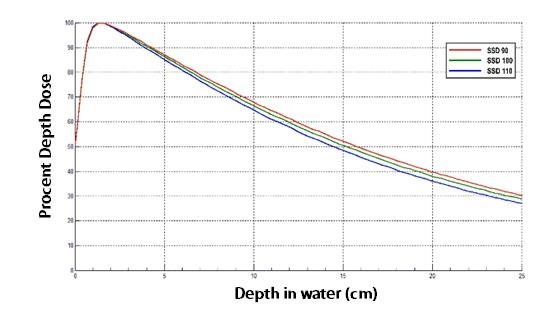
\includegraphics[width=0.8\textwidth]{figures/pdd}
		\caption{Percentage depth dose curve (water) for a 6 MV photon beam with 10
      x 10 cm field setup. Figure modified from Nurdin et al. \cite{Nurdin}.}
		\label{fig:pdd}
	\end{center}
\end{figure}
